\ifx\allfiles\undefined
\documentclass{article}
\usepackage{graphicx}
\usepackage{float}
\usepackage{geometry}
\usepackage{hyperref}
\usepackage{amssymb}
\usepackage{booktabs}
\usepackage{tabularx}
\usepackage{amsthm}
\usepackage{amsmath}
\usepackage{enumitem}
\usepackage{tikz}
\usetikzlibrary{shapes.geometric, automata, positioning, arrows, calc, arrows.meta}

\geometry{left=1.2in, right=1.2in, top=1.5in, bottom=1.5in}
\linespread{1.5}%行距

% 设置列表环境的上下间距
\setenumerate[1]{itemsep=5pt,partopsep=0pt,parsep=\parskip,topsep=5pt}
\setitemize[1]{itemsep=5pt,partopsep=0pt,parsep=\parskip,topsep=5pt}
\setdescription{itemsep=5pt,partopsep=0pt,parsep=\parskip,topsep=5pt}

\theoremstyle{definition}
\newtheorem{defn}{\textbf{\textit{def}}}[section]
\newtheorem{prop}{\textbf{\textit{prop}}}[section]
\newtheorem{thm}[defn]{\textbf{\textit{thm}}}
\newtheorem{corollary}[defn]{\textbf{\textit{corollary}}}
\newtheorem{lemma}[defn]{\textbf{\textit{lemma}}}
\newtheorem{criterion}[defn]{\textbf{\textit{criterion}}}
\newtheorem{claim}[defn]{\textbf{\textit{claim}}}

\newtheorem{example}{\textbf{\textit{e.g.}}}[section]
\newtheorem{exercises}{\textbf{\textit{exercises}}}[section]
\newtheorem*{remark}{\textbf{\textit{remark}}}

\newenvironment{solution}{\par{\textit{solution}}\;}{\qed\par}

\def\R{\mathbb{R}} % 实数域
\def\N{\mathbb{N}} % 自然数域
\def\Q{\mathbb{Q}} % 有理数域
\def\Z{\mathbb{Z}} % 整数域
\def\eps{\varepsilon} %ε

\def\bgtbl{\begin{table}[htbp]
    \centering
    \begin{tabularx}{\textwidth}{XXXXX}}
\def\bgpic{\begin{tikzpicture}[->,>=stealth',shorten >=1pt,auto,node distance=2.5cm,semithick]
    \tikzstyle{every state}=[fill=white,draw=black,text=black]}
\graphicspath{{pictures/},{../pictures/}}  % 配置图形文件检索目录
\begin{document}
\setcounter{section}{3}
\else
\fi
\section{Computability}

\textit{\textbf{Encoding of a multi-tape Turing Machine}: Assume our encoding of the TMs satisfy the following properties}

\begin{enumerate}
    \item \textit{Every string $\alpha\in\{0,1\}^*$ represents some TM (On invalid encoding $\alpha,M_{\alpha}$ always reject)}
    \item \textit{Every Turing Machine is represented by infinitely many strings}

    \textit{TM $M = (Q,\Sigma,\varGamma,\delta,q_0,q_{accept},q_{reject})$}
\end{enumerate}

\begin{thm}
    \textit{(Universal Turing Machine)}

    \textit{There exists a multitape Turing Machine $\mathcal{U}$, s.t. $\forall x,\alpha\in\{0,1\}^*,\mathcal{U}(x,\alpha) = M_\alpha(x)$. Moreover, if $M_\alpha$ halts on input x within T steps, then $\mathcal{U}(x,\alpha)$ halts in $O_M(T\log T)$ steps (weaker version $O_{M_\alpha}(T(n))^2$)}

    % \begin{proof}
    %     \textit{(for the weaker version)}

    %     \textit{By \textbf{lemma 3.9}, every multitape TM $M_\alpha$ can be converted to a single-tape TM $M_\beta$ within time $O_M(T^2)$}

    %     \textit{for each step of M, our UTM will:}

    %     \begin{enumerate}
    %         \item \textit{reads the symbol a on work tape of M}
    %         \item \textit{reads the current state $q_1$ of M}
    %         \item \textit{scans through the description of M to find $\delta(q_1,a)$}
    %         \item \textit{update the symbol (on the work tape of M), and moves the head if needed}
    %         \item \textit{updates "the current state of M" from $q_1$ to $q_2$}
    %     \end{enumerate}
        
    %     \textit{In total, the above simulation(for one step) takes $O(1)+O_M(1)+O_M(1)+O(1)+O_M(1) = O_M(1)$}
    % \end{proof}
\end{thm}    



\begin{lemma}
    \textit{Almost all languages are undecidable}

    \begin{proof}
        $\# languages = 2^{\aleph_0} = \aleph_1$

        $\#\{L\subseteq\{0,1\}^*\}$

        $\#TMs = \aleph_0$
    \end{proof}
\end{lemma}

\textit{thoughts: \textbf{diagonalization}}

$def~L_{flip} = \{\alpha:M_\alpha ~does~ not~ accept~ \alpha\}$


\begin{lemma}
    \textit{$L_{flip}$ is undecidable}
    \begin{proof}
        \textit{Assume for contradiction that $L_{flip}$ is decided by a TM $M_\beta$, which implies that $L(M_\beta) = L_{flip}$}

        \begin{itemize}
            \item \textit{case1: $\beta\in L_{flip}$. By definition $M_\beta$ does not accept $\beta$,i.e, $M_\beta$ rejects $\beta$. So, $\beta\notin L(M_\beta) = L_{flip}$. Contradiction!}
            \item \textit{case2: $\beta\notin L_{flip}$. By definition, $M_\beta$ accepts $\beta$. So, $\beta\in L(M_\beta) = L_{flip}$. Contradiction!}
        \end{itemize}
    \end{proof}
\end{lemma}

\textit{\\ \textbf{Turing halting problem}}

\textit{$L_{halt} = \{(\alpha,x),M_\alpha ~halts ~on ~x\}$}

\newpage
\textit{\\ \textbf{Fermat's Last Theorem}}

$(\forall m\geq 3)(\forall a,b,c\geq1)(a^m+b^m\neq c^m)$

$M_\alpha\begin{cases}
    T = 2\\
    while ~true\\
    T = T+1\\
    for ~d = 3 ~to~ T\\
    for~ a,b,c\in\{1,2,...,T\}\\
    if(a^d+b^d=c^d)\rightarrow exit\\
\end{cases}$

\textit{FLT iff $(M_\alpha,\eps)\notin L_{halt}$}

\textit{\\ \textbf{*reduction}}

\begin{defn}
    \textit{Let $L_1,L_2 \subseteq \{0,1\}^*$. Write $L_1\leq L_2$ if there is a reduction from $L_1$ to $L_2$ that, there exists a TM $M: \{0,1\}^*\rightarrow\{0,1\}^*$ (On any input x, M always halts and outputs a string M(x)), s.t.}
    \begin{enumerate}
        \item $(\forall x\in L_1)(M(x)\in L_2)$
        \item $(\forall x\notin L_1)(M(x)\notin L_2)$
    \end{enumerate}

    \textit{Let $L_1\leq L_2$ if $L_2$ is decidable, then $L_1$ is decidable.}

    \textit{contrpositive: If $L_1$ is undecidable, then $L_2$ is undecidable.}
\end{defn}

\begin{tikzpicture}
    % Draw rectangle
    \draw (0,0) rectangle (3,2);
    
    % Add arrow
    \draw[->, thick] (1.5,3) -- (1.5,2);
    \draw[->, thick] (1.5,0) -- (1.5,-1);
    
    % Add text
    \node at (1.5,1) {$M_2$};
    \node at (1.2,2.5) {$x$};
    \node at (1.5,-1.5) {$Yes/No$};
    \node at (-1.5,1) {$M_2~decides~L_2$};

    \draw[dashed] (5,0) rectangle (9,4);
    \draw (5.5,0.5) rectangle (8.5,1.5);
    \draw (5.5,2.5) rectangle (8.5,3.5);

    \draw[->, thick] (7,4.5) -- (7,3.5);
    \draw[->, thick] (7,2.5) -- (7,1.5);
    \draw[->, thick] (7,0.5) -- (7,-0.5);

    \node at (7,1) {$M_2$};
    \node at (7,3) {$M$};

    \node at (7.5,4.2) {$x$};
    \node at (7.5,2) {$M(x)$};
    \node at (7,-1) {$Yes/No$};
\end{tikzpicture}

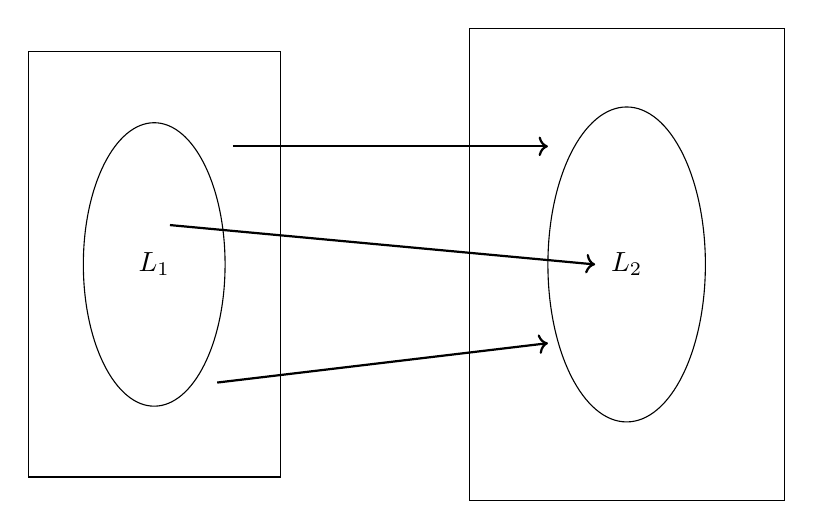
\begin{tikzpicture}
    \draw (0,0) ellipse (0.9cm and 1.8cm);
    \draw (6,0) ellipse (1cm and 2cm);
    \draw (-1.6,-2.7) rectangle (1.6,2.7);
    \draw (4,-3) rectangle (8,3);
    
    \node at (0,0) {$L_1$};
    \node at (6,0) {$L_2$};

    \draw[->, thick] (0.2,0.5) -- (5.6,0);
    \draw[->, thick] (1,1.5) -- (5,1.5);
    \draw[->, thick] (0.8,-1.5) -- (5,-1);
\end{tikzpicture}

\textit{If $x\in L_1$, then $M(x)\in L_2$, so $M_2$ accepts M(x)}

\textit{If $x\notin L_1$, then $M(x)\notin L_2$, so $M_2$ rejects M(x)}

\begin{thm}
    \textit{$L_{halt}$ is undecidable}

    \begin{proof}
        \textit{we will prove $L_{flip}\leq L'_{halt}$}

        \textit{Assuming $L_{halt}$ is decidable by a TM $M_{halt}$, we will prove $L_{flip}$ is decidable, which would be a contradiction.}
        
        \textit{Create a TM $M_{flip}$ as follows:}

        \textit{run $M_{halt}$ on input $(\alpha,\alpha)$}

        \begin{enumerate}
            \item \textit{If $M_{halt}$ rejects $(\alpha,\alpha)$, let $M_{flip}$ accept $\alpha$}
            \item \textit{If $M_{halt}$ accepts $\alpha,\alpha$, simulate $M_\alpha$ on input $\alpha$ (using a UTM), and flip the output}
        \end{enumerate}

        \textit{It is easy to verify $M_{flip}$ decides $L_{flip}$. Contradiction!}
    \end{proof}
\end{thm}

\begin{lemma}
    \textit{$L_{accept} = \{(\alpha,x)$, $M_\alpha$ accepts x\} is undecidable}

    \begin{proof}
        \textit{we will prove $L_{halt}\leq L_{accept}$. Assuming for contradiction that $L_{accept}$ is decidable, i.e. there exists a TM $M_{accept}$ that decides $L_{accept}$, we construct a TM $M_{halt}$ that decides $L_{halt}$ as follows:}
        \begin{enumerate}
            \item \textit{On input $(\alpha,x)$, create a new TM $M_\beta$, which simulates $M_\alpha$ on input x, and always accepts whenever $M_alpha$ halts (If $M_\alpha$ loops forever, $M_\beta$ loops forever as well)}
            \item \textit{Run $M_{accept}$ on input $(\beta,x)$, and forward its output. Clearly, $M_{halt}$ decides $L_{halt}$. Contradiction!} 
        \end{enumerate}
    \end{proof}
\end{lemma}

\begin{tikzpicture}
    % Draw rectangle
    \draw (0,0.5) rectangle (3,2.5);
    
    % Add arrow
    \draw[->, thick] (1.5,3.5) -- (1.5,2.5);
    \draw[->, thick] (1.5,0.5) -- (1.5,-0.5);
    
    % Add text
    \node at (1.5,1.5) {$M_{accept}$};
    \node at (1,3) {$(\alpha,x)$};
    \node at (1.5,-1) {$Yes/No$};
    \node at (1.5,-2) {$decides~if(\alpha,x)\in L_{accept}$};

    \draw[dashed] (5,0) rectangle (9,4);
    \draw (5.5,0.5) rectangle (8.5,1.5);
    \draw (5.5,2.5) rectangle (8.5,3.5);

    \draw[->, thick] (7,4.5) -- (7,3.5);
    \draw[->, thick] (7,2.5) -- (7,1.5);
    \draw[->, thick] (7,0.5) -- (7,-0.5);

    \node at (7,1) {$M_{accept}$};
    \node at (7,3) {$construct~B$};

    \node at (7.5,4.2) {$(\alpha,x)$};
    \node at (7.5,2) {$(\beta,x)$};
    \node at (7,-1) {$Yes/No$};
    \node at (10,2) {$M_{halt}$};
\end{tikzpicture}

\begin{lemma}
    \textit{Let $L_{empty}$ = \{$<M>$, M does not accept any input, i.e. $L(M) = \emptyset$\}}
    \begin{proof}
        \textit{We will prove $L_{halt}\leq L_{empty}$. Assuming for contradiction that $L_{empty}$ can be decided by a TM $M_{empty}$, we construct a TM $M_{halt}$ as follows:\\ On input $(\alpha,x)$}
        \begin{enumerate}
            \item \textit{We construct a new TM $M_\beta$, whose input is $y \in \{0,1\}^*$, as follows}
            \begin{enumerate}
                \item \textit{simulate $M_alpha$ on input x}
                \item \textit{if step (b) halts, always accept y}
            \end{enumerate}
            \textit{Clearly, $L(M_\beta) = \emptyset$ if $M_\alpha$ does not halt on x. Otherwise, $L(M_\beta) = \{0,1\}^*$}

            \item \textit{Run $M_{empty}$ on input $\beta$ and flip the output. We can verify that $M_{halt}$ decides $L_{halt}$. Contradiction!}
        \end{enumerate}
    \end{proof} 
\end{lemma}

\begin{tikzpicture}
    % Draw rectangle
    \draw (0,0.5) rectangle (3,2);
    
    % Add arrow
    \draw[->, thick] (1.5,3) -- (1.5,2);
    \draw[->, thick] (1.5,0.5) -- (1.5,-0.5);
    
    % Add text
    \node at (1.5,1.25) {$M_{empty}$};
    \node at (1,2.5) {$a$};
    \node at (1.5,-1) {$Yes/No$};
    

    \draw[dashed] (5,0) rectangle (9,4);
    \draw (5.5,0.5) rectangle (8.5,1.5);
    \draw (5.5,2.5) rectangle (8.5,3.5);

    \draw[->, thick] (7,4.5) -- (7,3.5);
    \draw[->, thick] (7,2.5) -- (7,1.5);
    \draw[->, thick] (7,0.5) -- (7,-0.5);
    \draw[->, thick] (7,-1.5) -- (7,-2.5);

    \node at (7,1) {$M_{empty}$};
    \node at (7,3.2) {$construct~M_\beta$};
    \node at (7,2.7) {$\beta = \beta(\alpha,x)$};

    \node at (7.5,4.2) {$(\alpha,x)$};
    \node at (7.5,2) {$\beta$};
    \node at (7,-1) {$Yes/No$};
    \node at (10,2) {$M_{halt}$};
    \node at (7,-3) {$No/Yes$};
\end{tikzpicture}

\begin{thm}
    \textit{Let $L_{regular}$ = \{$<M>$, M is a TM, s.t. L(M) is a regular language\}, it is decidable}
    \begin{proof}
        \textit{Assume for contradiction that $L_{regular}$ is decidable, i.e. $\exists$ a TM $M_{regular}$ that decides $L_{regular}$. We will prove $L_{accept}$ is decidable.}

        \textit{On input $(\alpha,x)$, construct a TM as follows:}

        \begin{enumerate}
            \item \textit{Construct a TM $M_\beta$, where $\beta = \beta(\alpha,x)$, and the input of $M_\beta$ is denoted by y}
            \begin{enumerate}
                \item \textit{If $y \in \{0^n1^n,n\geq0\}$, accept}
                \item \textit{Otherwise, simulate $M_\alpha$ on x, and accept iff $M_\alpha$ accepts x.}
            \end{enumerate}
            \item \textit{Run $M_{regular}$ on $\beta$, and forward its output}
            \begin{itemize}
                \item \textit{case1 $(\alpha,x)\notin L_{accept}$, i.e., $M_{alpha}$ does not accept x}
                
                \textit{So, $L(M_\beta) = \{0^n1^n,n\geq0\}$, which is not a regular language}

                \textit{Thus, $M_{regular}$ rejects $\beta$, which implies that $M_{halt}$ rejects $\beta$}

                \item \textit{case2 $(\alpha,x)\in L_{accept}$. So $L(M_\beta) = \{0,1\}^*$, which is regular}
                
                \textit{As such, $M_{regular}$ accepts $\beta$, and so does $M_{accept}$}
            \end{itemize}
        \end{enumerate}
    \end{proof}
\end{thm}

\begin{lemma}
    \textit{Let $L_{equal}$ = \{$(<M_1>,<M_2>)$, $M_1,M_2$ are TMs, s.t.  $L(M_1) = L(M_2)$\}, it's undecidable}

    \begin{proof}
        \textit{Assuming for contradiction that $L_{equal}$ is decidable, $L_{equal}$ is decided by a TM $M_{equal}$}

        \textit{On input $<M>$ construct a TM $M_{empty}$ as follows}

        \begin{enumerate}
            \item \textit{Run $M_{equal}$ on input $(<M>,<M_0>)$, where $M_0$ rejects immediately $(L(M_0) = \emptyset)$}
            \item \textit{Forward the above output}
        \end{enumerate}
    \end{proof}
\end{lemma}

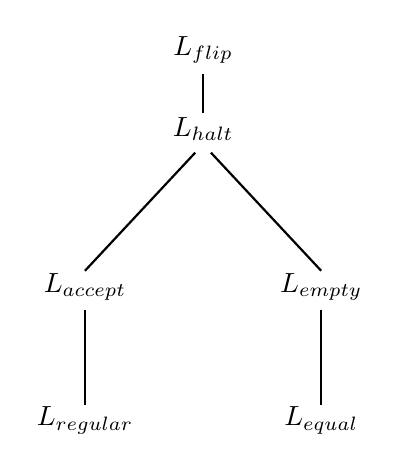
\begin{tikzpicture}
    \draw[thick] (0,7.2) -- (0,6.7);
    \draw[thick] (-0.1,6.2) -- (-1.5,4.7);
    \draw[thick] (0.1,6.2) -- (1.5,4.7);
    \draw[thick] (-1.5,4.2) -- (-1.5,3);
    \draw[thick] (1.5,4.2) -- (1.5,3);

    \node at (0,7.5) {$L_{flip}$};
    \node at (0,6.5) {$L_{halt}$};
    \node at (-1.5,4.5) {$L_{accept}$};
    \node at (1.5,4.5) {$L_{empty}$};
    \node at (-1.5,2.8) {$L_{regular}$};
    \node at (1.5,2.8) {$L_{equal}$};
\end{tikzpicture}

\ifx\allfiles\undefined
\end{document}
\fi